\section*{Maximum Power Transfer - AC}
	\begin{itemize}[noitemsep, nolistsep]
		\item $\mathbf{Z}_{Load}=\mathbf{Z}_{Th}^*$, $R_{Th}=\Re\lbrace\mathbf{Z_{Th}}\rbrace$, $R_L= \lvert \mathbf{Z}_{Th} \rvert = \sqrt{R_{Th}^2+\left( X_{Th}+X_{L}\right)^2}$
		\item $P_{max}=\frac{\lvert\mathbf{V}_{Th}\rvert^2}{8R_{Th}}$
	\end{itemize}
	\vspace{-4.5mm}
\section*{3-Phase Circuits} \label{sec:3-Phase}
	\begin{figure} % 3 Phase Configurations
		\begin{subfigure}{0.5\textwidth} % 3 Phase Y
			\centering
			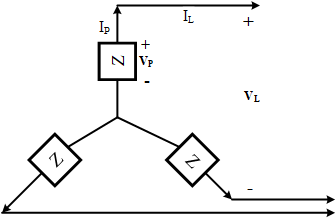
\includegraphics[scale=0.4]{3Phase-Y.png}
			\subcaption{\textbf{3 Phase $Y$-Connection}}
			\label{subfig:3 Phase-Y}
			\begin{align*}
				I_{L} &= I_{P} &
				V_{LL} &= \sqrt{3} V_{P} \angle \ang{30} &
				Z_{Y} &= \frac{Z_{\Delta}}{3} \\
				\mathbf{S} &= \sqrt{3} \mathbf{V}_{L} \mathbf{I}_{L}^{*} &
				\mathbf{S} &= 3 \mathbf{V}_{P} \mathbf{I}_{L}^{*} &
				\phi &= \theta_{V_{P}} - \theta_{I_{P}} \\
				\mathbf{S} &= S \angle \phi &
				P &= \lVert \mathbf{S} \rVert \cos \left( \phi \right) &
				Q &= \lVert \mathbf{S} \rVert \sin \left( \phi \right) \\
			\end{align*}
		\end{subfigure}
		\vline
		\begin{subfigure}{0.5\textwidth} % 3 Phase Delta
			\centering
			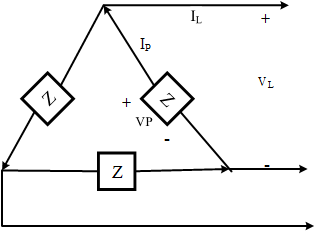
\includegraphics[scale=0.4]{3Phase-Delta.png}
			\subcaption{\textbf{3 Phase $\Delta$-Connection}}
				\begin{align*}
					I_{L} &= \sqrt{3} I_{P} \angle \ang{-30} &
					V_{LL} &= V_{P} &
					Z_{\Delta} &= 3 Z_{Y} \\
					\mathbf{S} &= \sqrt{3} \mathbf{V}_{L} \mathbf{I}_{L}^{*} &
					\mathbf{S} &= 3 \mathbf{V}_{P} \mathbf{I}_{P}^{*} &
					\phi &= \theta_{V_{P}} - \theta_{I_{P}} \\
					\mathbf{S} &= S \angle \phi &
					P &= \lVert \mathbf{S} \rVert \cos \left( \phi \right) &
					Q &= \lVert \mathbf{S} \rVert \sin \left( \phi \right) \\
				\end{align*}
			\label{subfig:3 Phase-Delta}
		\end{subfigure}
	\end{figure}
\begin{itemize}[noitemsep, nolistsep]
	\item $C_{Y} = \frac{Q_{C}}{3 \omega \lVert V_{\phi,rms} \rVert^{2}}$
	\item $C_{\Delta} = \frac{C_{Y}}{3}$
	\item Power lost due to line: $P_{Lost}=Z_{Wire}I_{L}$
\end{itemize}
You want to get everything into Y formation, because the common neutral allows you to do single-phase analysis.
\vspace{-5mm}